\section{Le prè-traitement}
\subsection{Le niveau de gris}
\textbf{Le concept}:\\
Une image se compose d'élément appelé pixel et definie par trois composante (en realite quattres mais ceci est une autre histoire) qui sont R,G et B correspondant au valeur Red, Green et Blue d'un pixel. Cette etape est primordiale car elle va permettre le bon traitement de l'image par l'ensemble des étapes aui la succède.\\
\textbf{La realisation}:\\
Pour réaliser ce niveau de gris on va travailler sur les trois composantes d'un pixel et appliquer la fromule suivante :
\\
\begin{center}
	\[x = \frac{0.299 \times R + 0.587 \times G + 0.114 \times B}{3}\]
\end{center}
à l'ensemble des pixels de l'image. Le niveau de gris est operationel dans notre ocr, nous pouvons donc passer à la tache suivante.
\begin{figure}[h]
	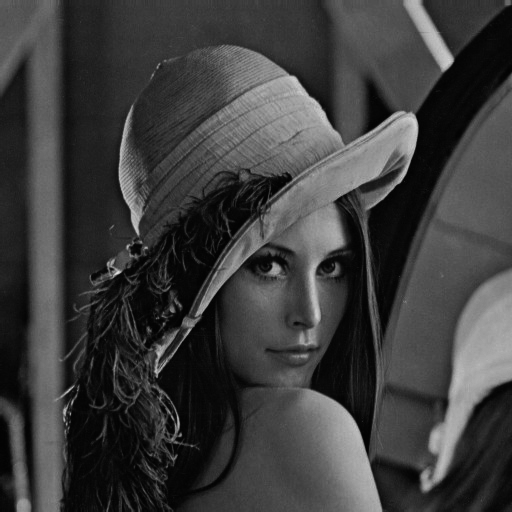
\includegraphics[width=0.50\textwidth]{grey.png}
	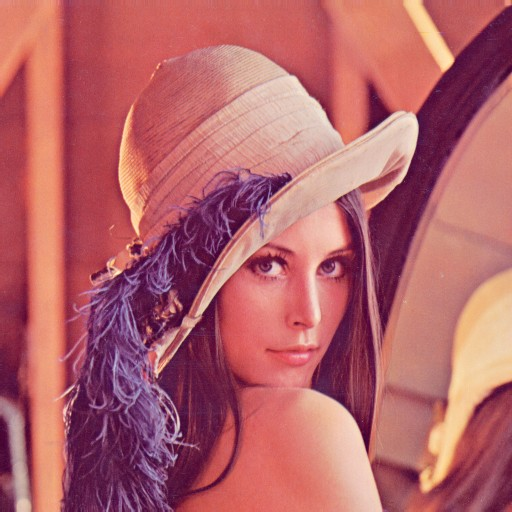
\includegraphics[width=0.50\textwidth]{lena.jpg}
	\caption{avec et sans nuance (captain obvious is obvious)}
\end{figure}
\newpage
\subsection{Le filtre median}
\textbf{Le concept}:\\
Le filtre median va pour chaque pixels de l'image recuperer le triplet (R,G,B) de chaque pixel autour du pixel traitré et trier ces pixels par ordre croissant. Il suffit juste de recuperer la valeur mediane de la liste trier. Le passe dans cette algo et qyue l'on doit passer les pixels sur une autre image pour pas fausser les calculs sur la premiere image !
\vspace{0.8cm}
\textbf{La realisation}:\\
En pratique ce filtre ne s'applique pas sur toute les images car sinon elle floute l'image et la rend intraitable. Je suis actuellement en recherche d'un algorithme permettant de palier ce gros probleme. Au niveau aulgoritemiaue on obtiens
\vspace{0.8cm}
\begin{figure}[h]
	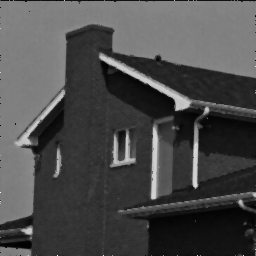
\includegraphics[width=0.50\textwidth]{house.png}
	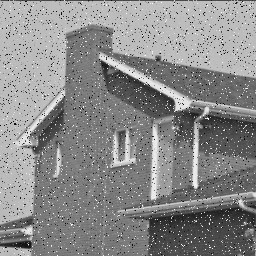
\includegraphics[width=0.50\textwidth]{house.jpg}
	\caption{presentation du filtre median}
\end{figure}
\newpage
\subsection{La binarisation}
\textbf{Le concept}:
Nous utilisons l'algorithme d'Otsu, du nom de son inventeur Nobuyuki Otsu. Qui se base sur l'histogramme d'un image. L'histogramme est un tableau de 255 element, ici des entiers, qui represente le nombre d'occurence d'un niveau de gris ( les niveau de gris allant de 0 (blanc) a 255 (noir). Dans un permier temps va creer un tableau pour y mettre les valeur traiter de l'histogramme de la maniere suivante
\begin{center}
	\[ p_{i} = \frac{h_{i}} {width * height}\]
\end{center}
qui renvoie la population du niveau de gris i dans l'ensemble des pixels de l'image.
Nous allons ensuite traiter tout les pixels de l'image en fonction de ce tableau et de deux autres formules magique ! qui sont pour un pixel k :\\
\begin{minipage}[h]{5cm}
	\begin{lstlisting}
	v = 0;
	for i = 0 to k do
	v = v + h.(i) * i
	done
	return v
	\end{lstlisting}
\end{minipage}
\begin{minipage}[h]{5cm}
	\begin{lstlisting}
	m = 0
	for i = 0 to k do
	m = m +. h.(i) * i
	done
	return m
	\end{lstlisting}
\end{minipage}
\vspace{0.8cm}
\\Le tout est injecter dans la formule

\[ s = v(i,p) \times (1 - v(i,p) \times (p.(255)) \times v(i,p) - m(i,p))^{2}\]
La methode de binarisation est plutot au point nous obtenons de tres bon resultats !
\begin{figure}[h]
	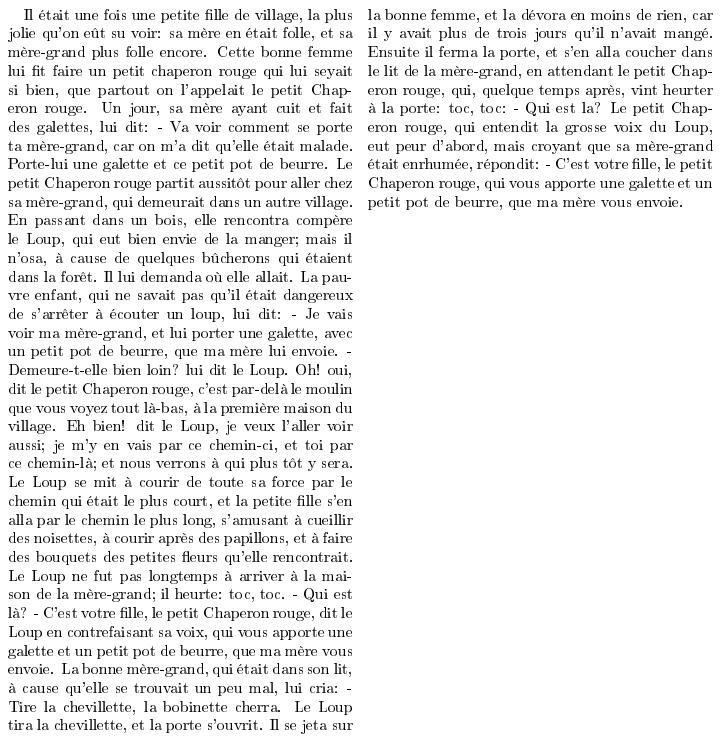
\includegraphics[width=0.50\textwidth]{bin.png}
	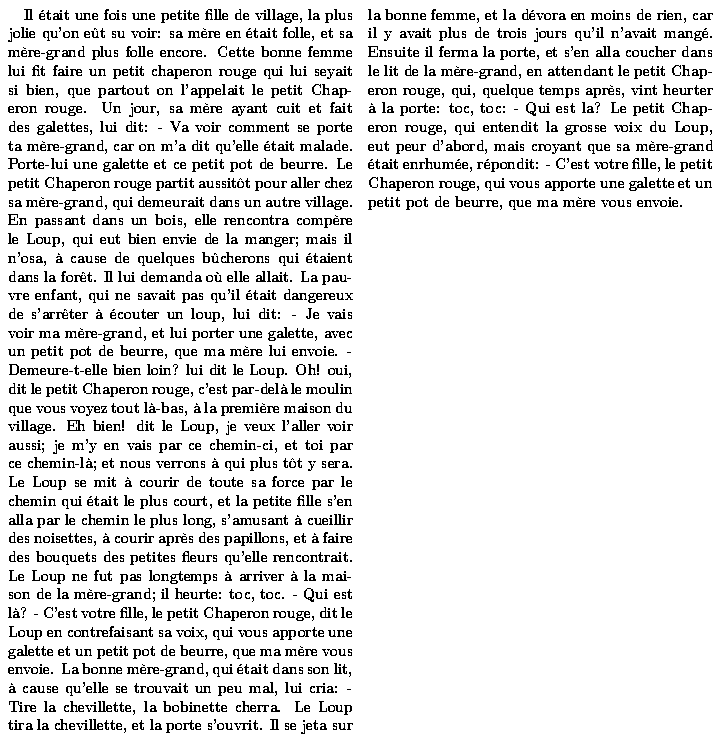
\includegraphics[width=0.50\textwidth]{bin2.png}
	\caption{exemple de binarisation}
\end{figure}

\subsection{la rotation d'image}
\subsubsection{Détection d'angle}
Je me suis donc occupe de la transformation de Hough. La transforme de hough est une techmiaue de reconnaissance de formes invente en 1962 par Paul Hough.
Le principe qui sous-tend la transforme de Hough est qu'il existe un nombre infini de ligne passant par un point dont la seule difference est l'orientation (l'angle). La transforme generalise de Houg fonctionne sur le principe qu'une droite peux s'ecrire sous la forme
\[r = x\cos{\theta}+y\sin{\theta}\]
A chaque pixels noir on essaye de trouver la vlauer maximum de r. Cette valeur represente la droite qui alligne le plus de pixel noir. On la retiens et on vote dans un tableau pour son angle associer. On recommence sur tout les pixels. L'angle qui a recu le plus de vote estl'anlge de rotation de l'image( minore de la moitier de l'intervalle pour pouvoir faire ressortir les angles negatifs).
\\
\newpage
Voici le principe de l'algo en pseudo code :
\begin{lstlisting}
for y =0 to hauteur de l'image do
for x =0 to largeur de l'image do
if (pixel noir ) then
angle = -Pi/2
while (angle < Pi/2) do
begin
r = x*cos(angle)+y*sin(angle)
if(r>o) then
/* increment tableau de vote */
angle ++
end
end
done
done

\end{lstlisting}

\begin{figure}[h]
	\centering
	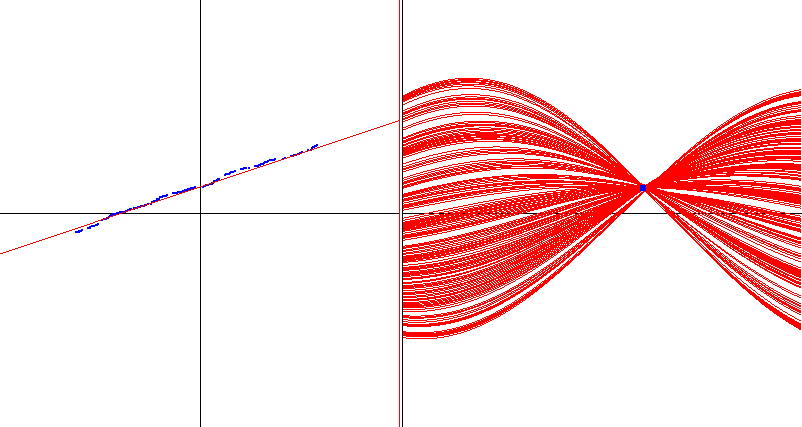
\includegraphics[width=0.80\textwidth]{hough.png}
\end{figure}
\newpage
\subsection{La rotation}
La rotation est effectue grace a une matrice de rotation. La methode consiste a assosicie chaque pixel (i, j) a une matrice [|[|i|]; [|j|]|] puis d'utilliser la formule suivate :
\\
\[A_{i,j}R_{\theta} = A'_{i,j} avec R = [|[|cos \theta; -sin \theta|]; [|sin \theta; cos \theta|]|] \]
\\
Le resultat sera alors de la forme [|[|i'|]; [|j'|]|], il faut alors creer une image d'une (diag, diag) avec diag la diagonal de l'image source, puis assigne la couleur du pixel (i, j) au pixel (i', j').
\subsection{Decoupage de l'image}
Le decoupage de l'image s'effectue en deux etapes, la premiere est de creer deux histogrammes, l'un representant le nombre de pixel noir sur sur chaque colonne et l'autre sur chaque ligne. Puis nous allons analyser chaque histogramme separement, l'histogramme va etre parcouru, et si le contenu est plus eleve qu'un certain seuil, la case sera considerer comme du texte, des premiers blocks vont donc etre forme, une fois ces blocks formees l'algorithme est reappele mais cette fois avec le deuxieme histogramme ce qui a pour effet de redecouper les blocks et d'enlever de plus en plus de parties blanches. Le processus est appele recursivement jusqu'a ce que les blocks aient la taille d'un charactere.
\subsection{Redimensionement de l'image }
Le redimensionement de l'image est utile pour pouvoir normaliser les caracteres a mettre en entre du reseau de neurone.En effet,toutes les entres du reseau de neurone doivent etre identique.Il est evident que tous les caracteres detecte par l'algorithme de XY-cut n'ont pas la meme taille.Il faut donc mettre a la meme taille tous les caracteres.Il existe plusieurs methode complexe et d'autre moins complexe mais qui provoquent souvent une baisse de la qualite de l'image.J'ai donc utilise une methode intermediaire : l'interpolation bilineaire.
Enfaite c'est assez simple, dans un premier temps on cree un ratio de largeur (x ratio = largeur de notre image/largeur attendue ) et un ratio de hauteur (y ratio= hauteur de l'image/hauteur attendue). On va cree une matrice correspondant a l'image de destination.A chaque image pixel de coodonne (x,y) de l'image attendue on va attribue les pixels de coordonne (x*x ratio,y * y ratio) de l'image source.
Voici l'algorithme en pseudo code :
\begin{lstlisting}
algorithme zoome (image src , entiers (w1,h2 )) /* dimension image attendue */
Debut
  image dst
  entier x_ratio = src.largeur/w2;
  entier y_ratio = src.hauteur/h2;
  pour x=0  a h2-1 faire
    pour y=0 a w2-1 faire
      dst(x,y) <-src(x_ratio*x,y_ratio*y);
    fin  pour
  fin pour
retourne dst; 
\end{lstlisting}
le probleme  est qu'avec cet algorithme nous creons ce qu'on appel de l'aliasing :
\begin{figure}[h]
    \centering
    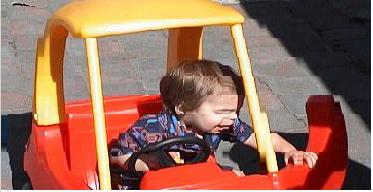
\includegraphics[width =0.80\textwidth]{aliasing.jpg}
\end{figure}
C'est a dire un trop grand contraste de couleur entre les differents pixels.Visuellement il apparait une forme d'escalier de gros contraste qui degrade fortement l'image. Le probleme de la qualite de l'image n'en est pas vraiment un pour nous.En effet nous travaillons sur des images binarises donc l aliasing cree des contrastes de blanc et de noir , ce qui a pour effet de parfois grossir certaines lettres.Ce probleme est a nouveau regle par le fait que l'on met en entre du reseau de neurone, uniquement le countoure des lettres (filtre laplacien) :
\begin{figure}[h]
    \centering
    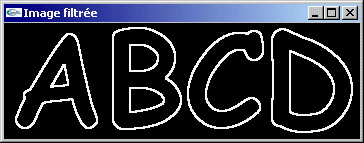
\includegraphics[width =0.80\textwidth]{ABCD.png}
\end{figure}

